\documentclass[tikz,border=10pt]{standalone}
\usepackage{amsmath}

\begin{document}
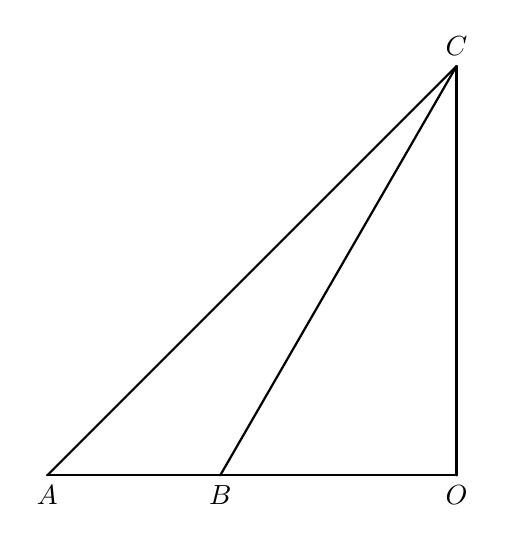
\begin{tikzpicture}[thick, >=stealth, scale=1.2, line join=round, line cap=round]
    % 依据解析计算所得参数建立精确坐标系
    % 设 OC = 25*sqrt(3) ≈ 43.3, 则 OB = OC/tan(60) = 25, OA = OC/tan(45) = 43.3
    % 为了绘图美观进行比例缩放
    \coordinate (O) at (4.33, 0);
    \coordinate (C) at (4.33, 4.33);
    \coordinate (B) at (1.83, 0); % OB = 25, 43.3-25=18.3 -> 1.83
    \coordinate (A) at (0, 0);

    % 1. 绘制水平面与树
    \draw (A) node[below] {$A$} -- (O) node[below] {$O$};
    \draw (O) -- (C) node[above] {$C$};
    
    % 2. 绘制视线
    \draw (A) -- (C);
    \draw (B) node[below] {$B$} -- (C);

\end{tikzpicture}
\end{document}